\documentclass{article}

% packages
\usepackage{amsmath, amsthm, thmtools, amsfonts, amssymb, luacode, catchfile, tikzducks, hyperref, ifthen}
\ifcsname c@kobocompile\endcsname
	\usepackage[a5paper, total={1072pt, 1448pt}, margin=10pt, includeheadfoot]{geometry} % set page margins
\else
	\usepackage[a4paper, margin=50pt, includeheadfoot]{geometry}
\fi
\usepackage[shortlabels]{enumitem}
\usepackage[skip=3pt, indent=0pt]{parskip}

% language
\usepackage[bidi=basic, layout=tabular, provide=*]{babel}
\ifcsname c@english\endcsname
	\babelprovide[main, import]{english}
\else
	\babelprovide[main, import]{hebrew}
	\babelprovide{rl}
\fi
%\babelfont{rm}{Libertinus Serif}
\babelfont{rm}[Renderer=Harfbuzz]{Libertinus Serif}
\babelfont{sf}{Libertinus Sans}
\babelfont{tt}{Libertinus Mono}

% style
\AddToHook{cmd/section/before}{\clearpage}	% Add line break before section
\linespread{1.3}
\setcounter{secnumdepth}{0}		% Remove default number tags from sections, this won't do well with theorems
\AtBeginDocument{\setlength{\belowdisplayskip}{3pt}}
\AtBeginDocument{\setlength{\abovedisplayskip}{3pt}}
\graphicspath{ {../images/} }

% operators
\DeclareMathOperator\cis{cis}
\DeclareMathOperator\Sp{Sp}
\DeclareMathOperator\tr{tr}
\DeclareMathOperator\im{Im}
\DeclareMathOperator\re{Re}
\DeclareMathOperator\diag{diag}
\DeclareMathOperator*\lowlim{\underline{lim}}
\DeclareMathOperator*\uplim{\overline{lim}}
\DeclareMathOperator\rng{rng}
\DeclareMathOperator\Sym{Sym}
\DeclareMathOperator\Arg{Arg}
\DeclareMathOperator\Log{Log}
\DeclareMathOperator\dom{dom}
\DeclareMathOperator\supp{Supp}
\DeclareMathOperator\var{Var}
\DeclareMathOperator\cov{Cov}

% commands
%\renewcommand\qedsymbol{\textbf{מש''ל}}
%\renewcommand\qedsymbol{\fbox{\emoji{lizard}}}
\newcommand{\Aa}[0]{\mathcal{A}}
\newcommand{\Bb}[0]{\mathcal{B}}
\newcommand{\CC}[0]{\mathbb{C}}
\newcommand{\Cc}[0]{\mathcal{C}}
\newcommand{\EE}[0]{\mathbb{E}}
\newcommand{\FF}[0]{\mathbb{F}}
\newcommand{\Ff}[0]{\mathcal{F}}
\newcommand{\Ii}[0]{\mathcal{I}}
\newcommand{\Gg}[0]{\mathcal{G}}
\newcommand{\Ll}[0]{\mathcal{L}}
\newcommand{\Mm}[0]{\mathcal{M}}
\newcommand{\NN}[0]{\mathbb{N}}
\newcommand{\Nn}[0]{\mathcal{N}}
\newcommand{\PP}[0]{\mathbb{P}}
\newcommand{\Pp}[0]{\mathcal{P}}
\newcommand{\QQ}[0]{\mathbb{Q}}
\newcommand{\RR}[0]{\mathbb{R}}
\newcommand{\Rr}[0]{\mathcal{R}}
\newcommand{\Ss}[0]{\mathcal{S}}
\newcommand{\TT}[0]{\mathbb{T}}
\newcommand{\Uu}[0]{\mathcal{U}}
\newcommand{\Vv}[0]{\mathcal{V}}
\newcommand{\Ww}[0]{\mathcal{W}}
\newcommand{\ZZ}[0]{\mathbb{Z}}
\newcommand{\acts}[0]{\circlearrowright}
\newcommand{\explain}[2] {
	\begin{flalign*}
		 && \text{#2} && \text{#1}
	\end{flalign*}
}
\newcommand{\maketitleprint}[0]{ \begin{center}
	%\begin{tikzpicture}[scale=3]
	%	\duck[graduate=gray!20!black, tassel=red!70!black]
	%\end{tikzpicture}	
	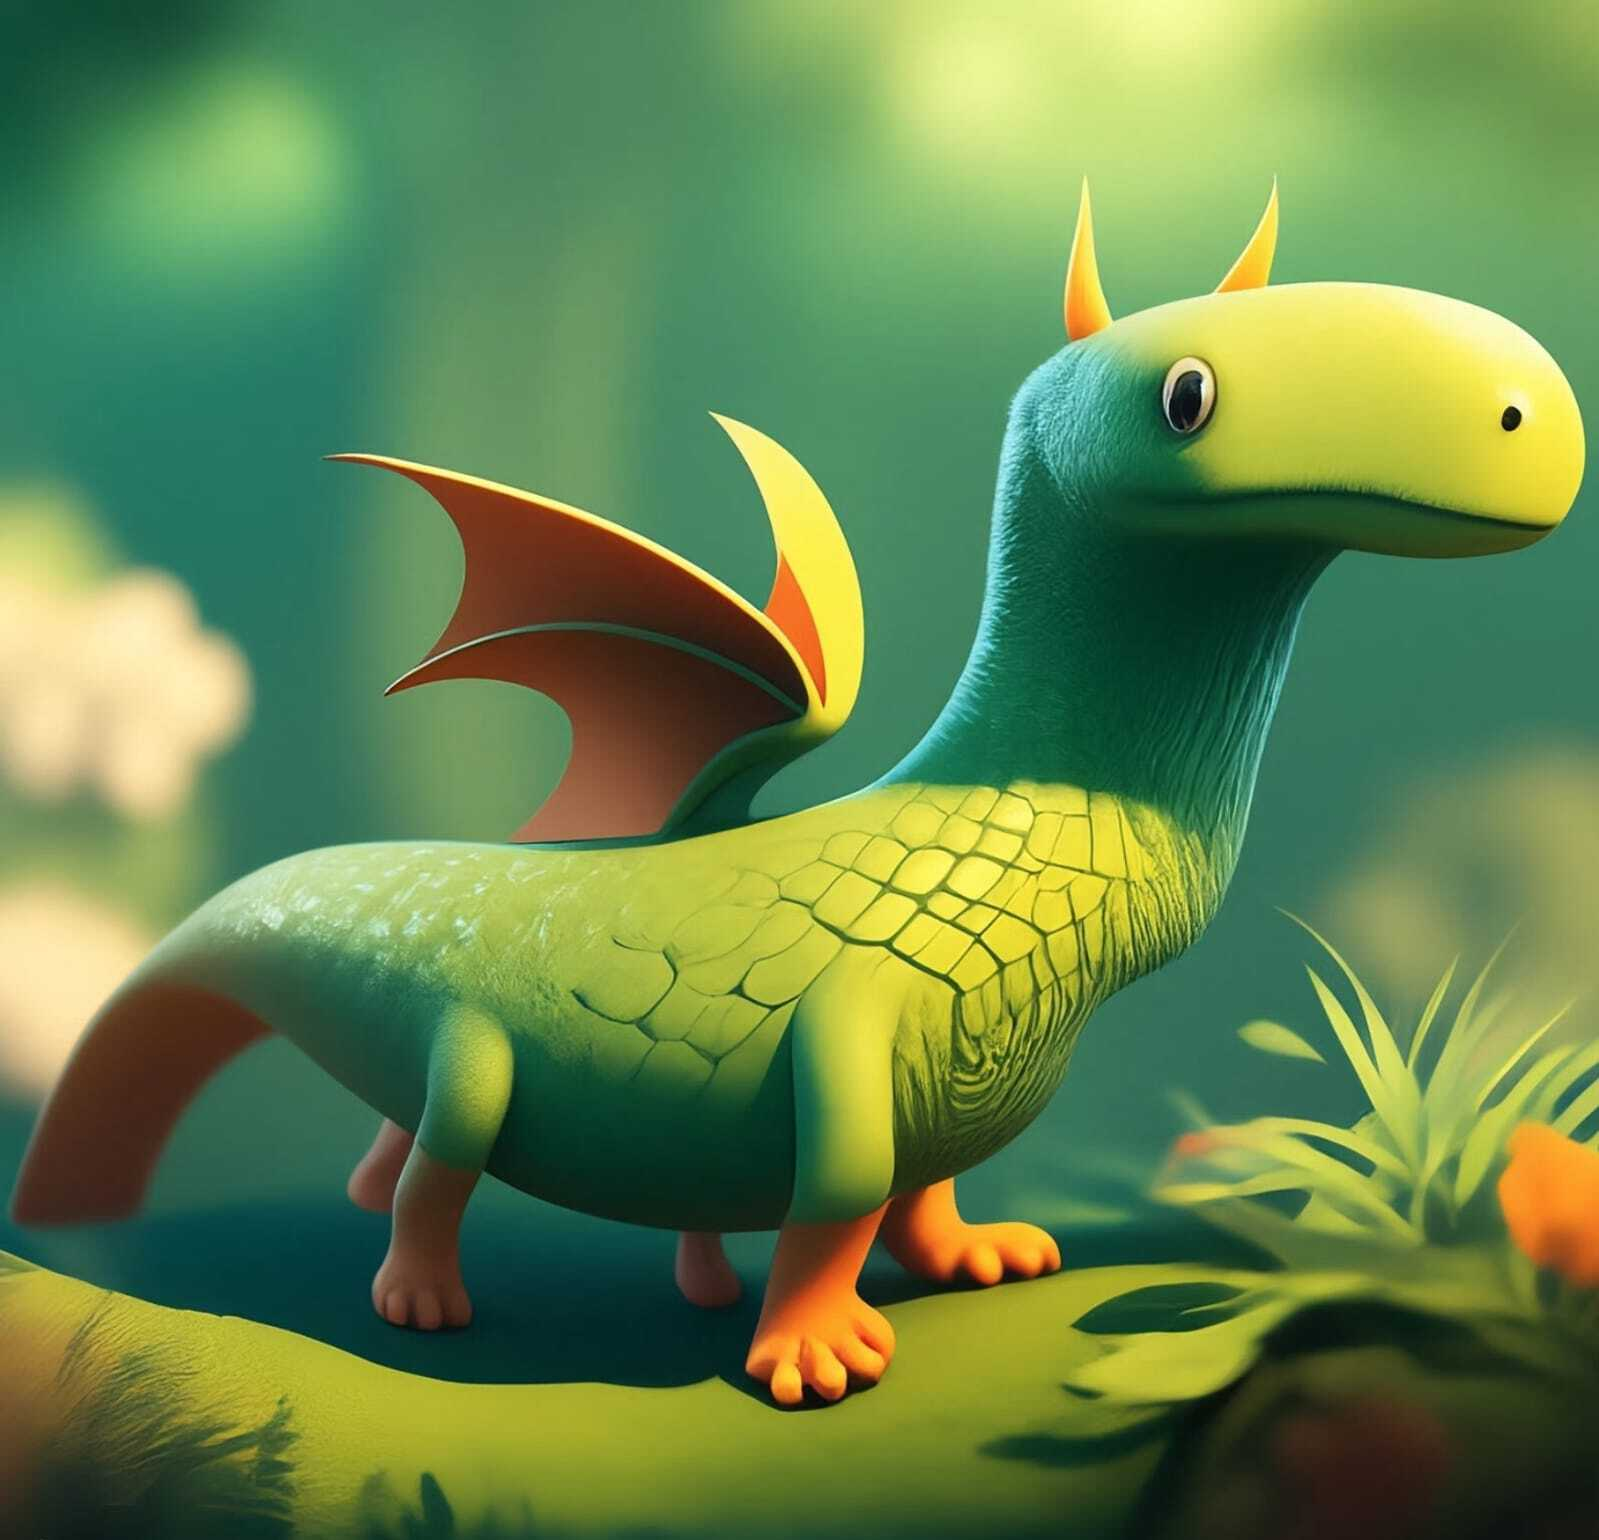
\includegraphics[width=6cm]{cover}
\end{center}
}

% theorem commands
\newtheoremstyle{c_remark}
	{}	% Space above
	{}	% Space below
	{}% Body font
	{}	% Indent amount
	{\bfseries}	% Theorem head font
	{}	% Punctuation after theorem head
	{.5em}	% Space after theorem head
	{\thmname{#1}\thmnumber{ #2}\thmnote{ \normalfont{\text{(#3)}}}}	% head content
\newtheoremstyle{c_definition}
	{3pt}	% Space above
	{3pt}	% Space below
	{}% Body font
	{}	% Indent amount
	{\bfseries}	% Theorem head font
	{}	% Punctuation after theorem head
	{.5em}	% Space after theorem head
	{\thmname{#1}\thmnumber{ #2}\thmnote{ \normalfont{\text{(#3)}}}}	% head content
\newtheoremstyle{c_plain}
	{3pt}	% Space above
	{3pt}	% Space below
	{\itshape}% Body font
	{}	% Indent amount
	{\bfseries}	% Theorem head font
	{}	% Punctuation after theorem head
	{.5em}	% Space after theorem head
	{\thmname{#1}\thmnumber{ #2}\thmnote{ \text{(#3)}}}	% head content

\ifcsname c@english\endcsname
	\theoremstyle{plain}
	\newtheorem{theorem}{Theorem}[section]
	\newtheorem{lemma}[theorem]{Lemma}
	\newtheorem{proposition}[theorem]{Proposition}
	\newtheorem*{proposition*}{Proposition}
	%\newtheorem{corollary}[theorem]{אין חלופה עברית}

	\theoremstyle{definition}
	\newtheorem{definition}[theorem]{Definition}
	\newtheorem*{definition*}{Definition}
	\newtheorem{example}{Example}[section]
	\newtheorem{exercise}{Exercise}[section]

	\theoremstyle{remark}
	\newtheorem*{remark}{Remark}
	\newtheorem*{solution}{Solution}
	\newtheorem{conclusion}[theorem]{Conclusion}
	\newtheorem{notation}[theorem]{Notation}
\else
	\theoremstyle{c_plain}
	\newtheorem{theorem}{משפט}[section]
	\newtheorem{lemma}[theorem]{למה}
	\newtheorem{proposition}[theorem]{טענה}
	\newtheorem*{proposition*}{טענה}
	%\newtheorem{corollary}[theorem]{אין חלופה עברית}

	\theoremstyle{c_definition}
	\newtheorem{definition}[theorem]{הגדרה}
	\newtheorem*{definition*}{הגדרה}
	\newtheorem{example}{דוגמה}[section]
	\newtheorem{exercise}{תרגיל}[section]

	\theoremstyle{c_remark}
	\newtheorem*{remark}{הערה}
	\newtheorem*{solution}{פתרון}
	\newtheorem{conclusion}[theorem]{מסקנה}
	\newtheorem{notation}[theorem]{סימון}
\fi

% Questions related commands
\newcounter{question}
\setcounter{question}{1}
\newcounter{sub_question}
\setcounter{sub_question}{1}

\ifcsname c@english\endcsname
	\newcommand{\question}[1][0]{
		\ifthenelse{#1 = 0}{}{\setcounter{question}{#1}}
		\section{Question \arabic{question}}
		\addtocounter{question}{1}
		\setcounter{sub_question}{1}
	}

	\newcommand{\subquestion}[1][0]{
		\ifthenelse{#1 = 0}{}{\setcounter{sub_question}{#1}}
		\subsection{Part \alph{sub_question}}
		\addtocounter{sub_question}{1}
	}
\else
	\newcommand{\question}[1][0]{
		\ifthenelse{#1 = 0}{}{\setcounter{question}{#1}}
		\section{שאלה \arabic{question}}
		\addtocounter{question}{1}
		\setcounter{sub_question}{1}
	}

	\newcommand{\subquestion}[1][0]{
		\ifthenelse{#1 = 0}{}{\setcounter{sub_question}{#1}}
		\subsection{סעיף \localecounter{letters.gershayim}{sub_question}}
		\addtocounter{sub_question}{1}
	}
\fi

% import lua and start of document
\directlua{common = require ('../common')}

\GetEnv{AUTHOR}

% headers
\author{\AUTHOR}
\date\today

\title{פתרון מטלה 1 – חשבון אינפיניטסימלי 2 (80132--2)}

\begin{document}
\maketitle
\maketitleprint{}

\section{שאלה 1}
\subsection{סעיף א'}
נוכיח כי הפונקציה $f(x) = x^3 + 5x^2 + 1$ גזירה בנקודה $x_0 = 3$. \\*
על־פי הגדרת הנגזרת הגבול הבא צריך להתקיים:
\begin{align*}
	& \lim_{h \to 0} \frac{f(3 + h) - f(3)}{h} \\
	= & \lim_{h \to 0} \frac{1}{h} ({(3 + h)}^3 + 5{(3 + h)}^2 + 1 - 3^3 - 5 \cdot 3^2 - 1) \\
	= & \lim_{h \to 0} \frac{1}{h} ({(3 + h)}^3 + 5{(3 + h)}^2 - 72) \\
	= & \lim_{h \to 0} \frac{1}{h} (3^3 + 3 \cdot 3^2 h + 3 \cdot 3^1 h^2 + h^3 + 5\cdot 3^2 + 5 \cdot 6h + 5h^2 - 72) \\
	= & \lim_{h \to 0} \frac{1}{h} (27 h + 9 h^2 + h^3 + 30h + 5h^2) \\
	= & \lim_{h \to 0} 57 + 14 h + h^2 \\
	= & 57 + 14 \cdot 0 + 0^2 = 57
\end{align*}
מצאנו כי הגבול מתקיים ולכן הפונקציה גזירה בנקודה ואף מתקיים $\left. \frac{df}{dx}\middle\vert_{x = x_0}\right. = 57$.

\subsection{סעיף ב'}
נוכיח כי הפונקציה $f(x) = \sqrt[3]{x}$ גזירה בנקודה $x_0 = 2$:
\begin{proof}
	נגזרת מוגדרת בנקודה אם ורק אם הגבול הבא מתקיים:
	\begin{align*}
		& \lim_{h \to 0} \frac{1}{h} \left(\sqrt[3]{2 + h} - \sqrt[3]{2}\right) \\
		= & \lim_{h \to 0} \frac{1}{h} \left(\sqrt[3]{2 + h} - \sqrt[3]{2}\right) \frac{\sqrt[3]{{(2 + h)}^2} + \sqrt[3]{2(2 + h)} + \sqrt[3]{2^2}}{\sqrt[3]{{(2 + h)}^2} + \sqrt[3]{2(2 + h)} + \sqrt[3]{2^2}} \\
		= & \lim_{h \to 0} \frac{1}{h} \frac{2 + h - 2}{\sqrt[3]{{(2 + h)}^2} + \sqrt[3]{2(2 + h)} + \sqrt[3]{2^2}} \\
		= & \lim_{h \to 0} \frac{1}{\sqrt[3]{{(2 + h)}^2} + \sqrt[3]{2(2 + h)} + \sqrt[3]{2^2}} \\
		= & \frac{1}{\sqrt[3]{{(2 + 2)}^2} + \sqrt[3]{2(2 + 2)} + \sqrt[3]{2^2}} \\
		= & \frac{1}{3 \sqrt[3]{4}}
	\end{align*}
	מצאנו כי הגבול מתקיים ולכן נובע כי $f'(2) = \frac{1}{3 \sqrt[3]{4}}$.
\end{proof}

\subsection{סעיף ג'}
נראה את הטענה כי הפונקציה $f(x) = \lfloor x \rfloor$ גזירה בכל נקודה $x_0 \in \RR$ על־ידי דוגמה נגדית:
נגדיר $x_0 \in \ZZ$, ידוע כי הפונקציה $f$ איננה רציפה בנקודות $x_0$, ולכן עומדת בסתירה לטענה כי הן גזירות בנקודה זו.

\section{שאלה 2}
תהי $f$ פונקציה המוגדרת על־ידי
\[
	f(x) = \begin{cases}
		-x & 0 \le x \\
		1 & x < 0
	\end{cases}
\]

\subsection{סעיף א'}
נראה כי הפונקציה גזירה מימין בנקודה $x_0 = 0$: \\*
לכל סביבה ימנית של $0$ ב־$f$ מתקיים $f(x) = -x$, ואנו כמובן יודעים כי ביטוי זה גזיר וערך נגזרתו הוא $-1$, לכן נסיק כי גם $f$ גזירה מימין בנקודה.

\subsection{סעיף ב'}
נחשב את הפונקציה $f \circ f$: \\*
עבור $x < 0$ נקבל $f(x) = 1$ ובהתאם $f(1) = -1$ ולכן $(f \circ f)(x) = -1$. \\*
עבור $0 < x$ נקבל $f(x) = -x$, ובהתאם $f(-x) = 1$ ולכן $(f \circ f)(x) = 1$. \\*
לבסוף נחשב $f(f(0)) = f(0) = 0$:
\[
	f \circ f = \begin{cases}
		-1 & x < 0 \\
		0 & x = 0 \\
		1 & x > 0
	\end{cases}
\]

\subsection{סעיף ג'}
תהי פונקציה $g$ אשר מוגדרת בסביבה מלאה של $x_0 \in \RR$, וגזירה מימין בנקודה, ותהי פונקציה $h$ המוגדרת בסיבבה מלאה של $x_1 = g(x_0)$ וגזירה מימין ב־$x_1$.
נוכיח כי $h \circ g$ גזירה מימין אף היא בנקודה $x_0$:
\begin{proof}
	הלכה למעשה טענה זו נובעת ישירות ממשפט הרכבת פונקציות בגבולות חלקיים. \\*
	ידוע כי $g$ גזירה מימן ולכן גם רציפה מימין בנקודה ולכן
	\[
		\lim_{x \to x_0^+} g(x) = g(x_0) = x_1,
		\lim_{x \to x_1^+} \frac{h(x) - h(x_1)}{x - x_1}
	\]
	נשתמש במשפט ההרכבה:
	\[
		\lim_{g(x) \to x_1^+} \frac{h(g(x)) - h(g(x_0))}{x - g(x_0)}
		= \lim_{x \to x_1^+} \frac{h(g(x)) - h(g(x_0))}{x - g(x_0)}
	\]
	והגבול כמובן מוגדר
\end{proof}

\section{שאלה 3}
\subsection{סעיף א'}
\begin{align*}
	& \lim_{h \to 0} \frac{f(x_0 - 2h) - f(x_0 + 3h)}{h} \\
	= & \lim_{h \to 0} \frac{f(x_0 - 2h) - f(x_0) + f(x_0) - f(x_0 + 3h)}{h} \\
	= & \lim_{h \to 0} 2 \frac{f(x_0 - 2h) - f(x_0)}{2h} - 3 \frac{ f(x_0 + 3h) - f(x_0)}{3h} \\
	= & 2f'(x_0) - 3f'(x_0) = -f'(x_0)
\end{align*}

\subsection{סעיף ב'}
נגדיר את הפונקציה $g(x) = |x|$ ונבחן את הנקודה $x_0 = 0$. \\*
אנו כבר יודעים כי הפונקציה איננה גזירה בנקודה זו, למרות זאת מתקיים:
\[
	\lim_{h \to 0} \frac{g(0 + h) - g(0 - h)}{2h}
	= \lim_{h \to 0} \frac{|h| - |-h|}{2h}
	= \lim_{h \to 0} \frac{|h| - |h|}{2h}
	= 0
\]
דהינו, הגבול מתקיים וערכו $0$ בסתירה לאי־קיום הנגזרת בנקודה זו.

\section{שאלה 4}
תהינה $f, g$ פונקציות המוגדרות בסביבה של $x_0 \in \RR$.

\subsection{סעיף א'}
נוכיח כי אם $f(x_0) = g(x_0)$ וגם $f_-'(x_0) = g_+'(x_0)$ אז הפונקציה $h(x) = \begin{cases}
	f(x) & x < x_0 \\
	g(x) & x \ge x_0
\end{cases}$ גזירה ב־$x_0$:
\begin{proof}
	הפונקציה $h$ מתלכדת בסביבתה הימנית עם $g$ ובשמאלית עם $f$ ולכן מתקיימים הגבולות:
	\[
		\lim_{x \to x_0^-} \frac{h(x) - h(x_0)}{x - x_0}
		= \lim_{x \to x_0^-} \frac{f(x) - f(x_0)}{x - x_0}
		= f'_-(x_0)
		= g'_+(x_0)
		= \lim_{x \to x_0^+} \frac{g(x) - g(x_0)}{x - x_0}
		= \lim_{x \to x_0^+} \frac{h(x) - h(x_0)}{x - x_0}
	\]
	וקיבלנו כי $h'(x_0)$ מוגדרת שכן שני הגבולות החלקיים מתכנסים לאותו ערך ולכן גם הגבול הכללי מתקיים.
\end{proof}

\subsection{סעיף ב'}
נפריך את הטענה כי אם $fg$ ו־$f$ גזירות בנקודה $x_0$ אז גם $g$ גזירה בנקודה זו על־ידי דוגמה נגדית: \\*
נגדיר $f(x) = 0$ ו־$g(x) = |x|$, $x_0 = 0$. \\*
כמובן שמתקיים $f(x) g(x) = 0$ לכל $x$ בתחום הגדרתן, וברור כי $f'(0) = 0$, אך $g$ איננה גזירה ב־$x_0 = 0$.

\subsection{סעיף ג'}
נסתור את הטענה כי אילו $f, g : \RR \rightarrow \RR$ וגם $f$ לא גזירה ב־$x_0$ ו־$g$ גזירה בכל נקודה אז $g \circ f$ איננה גזירה ב־$x_0$ עם דוגמה נגדית. \\*
נגדיר שוב $g(x) = 0$ ו־$f(x) = |x|$ עבור $x_0 = 0$. ברור למה תנאי הטענה מתקיימים אך כמובן $g \circ f = 0$ לכל $x \in \RR$ ולכן גם גזירה בתחום זה.

\section{שאלה 5}
תהי $h$ פונקציה גזירה בנקודה $x_0 \in \RR$.
\subsection{סעיף א'}
נתון כי קיימת $\delta > 0$ כך שמתקיים $h(x_0) < h(x)$ לכל $x \in (x_0, x_0 + \delta)$. \\*
נוכיח כי $0 \le h'(x_0)$
\begin{proof}
	נניח בשלילה כי $h'(x_0) < 0$. לכן מתקיים
	\[
		\lim_{x \to x_0^+} \frac{h(x) - h(x_0)}{x - x_0} < 0
	\]
	על־פי הגדרת הגבול הנתון, נובע כי ל־$\epsilon = \delta$ קיים $\delta_0$ כך שלכל $x \in \RR$ המקיים $0 < x - x_0 < \delta_0$ מתקיים
	\[
		\frac{h(x) - h(x_0)}{x - x_0} < 0 \land x - x_0 \implies h(x) - h(x_0) < 0 \implies h(x) < h(x_0)
	\]
	בסתירה לטענה, לכן לא מתקיים $h'(x_0) < 0$ ובהתאם נובע כי $h'(x_0) \ge 0$.
\end{proof}

\subsection{סעיף ב'}
נניח כי $h'(x_0) > 0$ ונוכיח $\exists \delta : \forall x \in (x_0, x_0 + \delta) : h(x) > h(x_0)$.
\begin{proof}
	למעשה, זוהי הוכחה דומה להוכחה של הסעיף הקודם, מתקיים הגבול החד־צדדי:
	\[
		h'_+(x_0) = \lim_{x \to x_0^+} \frac{h(x) - h(x_0)}{x - x_0} > 0
	\]
	נבחר $\epsilon > 0$ אשר עבורו נתונה $\delta_0$ עבורה לכל $x \in \RR$ המקיים $0 < x - x_0 < \delta_0$ מתקיים:
	\[
		\frac{h(x) - h(x_0)}{x - x_0} > 0 \implies h(x) - h(x_0) > 0 \implies h(x) > h(x_0)
	\]
	ולבסוף נגדיר $\delta = \delta_0$. \\*
	את הכיוון ההפוך נוכיח באותה הדרך בדיוק עבור הפונקציה $h^*(x) = -h(x)$ והנקודה $x_1 = -x_0$, ונראה כי הטענה מתקיימת במלואה.
\end{proof}

\section{שאלה 6}
\subsection{סעיף א'}
יהי $n \in \NN$ ותהי $f_n : \RR \to \RR$ המוגדרת על־ידי $f_n(x) = x^n$. \\*
נוכיח כי $f_n$ גזירה ב־$x_0 \in \RR$ וכי $f_n'(x_0) = nx_0^{n + 1}$.
\begin{proof}
	נבחן את הגדרת הנגזרת:
	\begin{align*}
		& \lim_{h \to 0} \frac{1}{h} \left( f_n(x_0 + h) - f_n(x_0) \right) \\
		= & \lim_{h \to 0} \frac{1}{h} \left( {(x_0 + h)}^n - x_0^n \right) \\
		\text{פירוק בינומי} = & \lim_{h \to 0} \frac{1}{h} \left( \left(\sum_{i = 0}^{n} \binom{n}{i} x_0^i  h^{n - i}\right) - x_0^n \right) \\
		= & \lim_{h \to 0} \frac{1}{h}  \left(\sum_{i = 0}^{n - 1} \binom{n}{i} x_0^i  h^{n - i}\right)  \\
		= & \lim_{h \to 0} \sum_{i = 0}^{n - 1} \binom{n}{i} x_0^i  h^{n - i - 1}  \\
		\text{סכום סופי ואריתמטיקה של גבולות} = & \sum_{i = 0}^{n - 1} \lim_{h \to 0} \binom{n}{i} x_0^i  h^{n - i - 1}  \\
		= & \binom{n}{n - 1} x^{n - 1} + \sum_{i = 0}^{n - 2} \binom{n}{i} x_0^i  0^{n - i - 1}  \\
		f_n'(x_0) = & n x^{n - 1}
	\end{align*}
\end{proof}

\subsection{סעיף ב'}
יהי $n \in \ZZ$ ותהי $f_n : \RR \setminus \{0\}$ המוגדרת על־ידי $f_n(x) = x_n$. \\*
נוכיח כי $f_n$ גזירה בנקודה $x_0 \in \RR \setminus \{0\}$ ואף $f_n'(x_0) = nx_0^{n - 1}$.
\begin{proof}
	אילו $n > 0$ אז מתקיים $n \in \NN$, והטענה מתקיימת על־פי הסעיף הקודם, לכן נניח כי $n < 0$. \\*
	נגדיר $m = -n$ ונראה כי מתקיים $f_n(x) = \frac{1}{x^m}$ לכל $n < 0$.
	\begin{align*}
		& \lim_{h \to 0} \frac{1}{h} \left( f_n(x_0 + h) - f_n(x_0) \right)
		& = \lim_{h \to 0} \frac{1}{h} \left( \frac{1}{{(x_0 + h)}^m} - \frac{1}{x_0^m} \right) \\
		& = \lim_{h \to 0} \frac{x_0^m - {(x_0 + h)}^m}{h \, x_0^m {(x_0 + h)}^m}
		& = \lim_{h \to 0} \frac{-\sum_{i = 0}^{m - 1} \binom{m}{i} x_0^i  h^{m - i - 1}}{x_0^m {(x_0 + h)}^m} \\
		& = \lim_{h \to 0} \frac{-m x^{m - 1} - h \sum_{i = 0}^{m - 2} \binom{m}{i} x_0^i  h^{m - i - 1}}{x_0^m {(x_0 + h)}^m}
		& = \frac{-m x^{m - 1} + 0}{x_0^m {(x_0 + 0)}^m} \\
		& = \frac{-m x^{m - 1}}{x_0^{2m}} = \frac{m}{x_0^{m + 1}} = nx_0^{n - 1}
	\end{align*}
\end{proof}

\section{שאלה 7}
\subsection{סעיף א'}
יהי $0 < x \in \RR$, נוכיח כי קיים $n \in \ZZ$ יחיד כך שמתקיים $10^n \le x < 10^{n + 1}$.
\begin{proof}
	נשים לב כי הקטע $[10^n, 10^{n + 1})$ מייצג את הקטע מהטענה, ונשים לב כי %chktex 9
	\[
		\bigcap_{n = -\infty}^{\infty} [10^n, 10^{n + 1}) = (-\infty, \infty) %chktex 9
	\]
	את הטענה ניתן להוכיח בקלות באינדוקציה, לכן בוודאי $x \in (-\infty, \infty)$. \\*
	נניח בשלילה כי ישנם שני $n < n_0$ המקיימים את הטענה, לכן $10^n \le x < 10^{n + 1} \land 10^{n_0} \le x < 10^{n_0 + 1}$. \\*
	נשים לב גם כי $10^n < 10^{n_0}$ ובהתאם $10^{n + 1} \le 10^{n_0}$. ונקבל כי $x < 10^{n + 1} \le x$, לכן בהכרח אין שני $n$־ים שונים המקיימים את הטענה.
\end{proof}

\subsection{סעיף ב'}
עבור $0 < x \in \RR$ נוכיח כי קיימים $n \in \ZZ$, ו־$x' \in [0, 1)$ יחידים כך ש־$\log_{10}(x) = n + x'$. %chktex 9
\begin{proof}
	נראה כי מתקיים $n \le \log_{10}(x) < n + 1$ על־פי החלק השלם $\lfloor n + x' \rfloor = n$. \\*
	בהתאם מתקיים גם $10^n \le 10^{\log_{10}(x)} = x < 10^{n + 1}$, וטענה זו נכונה על־פי הסעיף הקודם.
\end{proof}

\subsection{סעיף ג'}
בסעיף א' הוכחנו את הטענה אשר חוסמת כל מספר במספר הקטן ביותר בעל אותה כמות ספרות כמוהו והמספר הגדול ביותר עם כמות הספרות הזו, היא $n + 1$.
כמובן הסיבה היא שהמספר הוא $n + 1$ היא שהכפלה ב־$10$ מוסיפה ספרה, וכאשר האיבר הנייטרלי לחיבור לא מוכפל בעשר כלל, הוא עדיין מצריך ספרה יחידה לכתיבה. \\*
בסעיף ב' מצאנו כי $\lfloor \log_{10}(x) \rfloor = n$, לכן בהתאם כמות הספרות במספר $x$ היא $\lfloor \log_{10}(x) \rfloor + 1$.

\subsection{סעיף ד'}
\[
	10^5 \le 493566 < 10^6 \implies 5 \le \log_{10}(493566) < 6
\]
לכן הערך הוא בערך $5$ או $6$.

\end{document} %chktex 17
